%-----------------------------------------------------------------------
% Beginning of chapter.tex
%-----------------------------------------------------------------------
%
%  This is a sample file for use with AMS-LaTeX.  It provides an example
%  of how to set up a file for a book to be typeset with AMS-LaTeX.
%
%  This is the driver file.  Separate chapters should be included at
%  the end of this file.
%
%  ***** DO NOT USE THIS FILE AS A STARTER FOR YOUR BOOK. *****
%  Follow the guidelines in the file chapter.template.
%
%%%%%%%%%%%%%%%%%%%%%%%%%%%%%%%%%%%%%%%%%%%%%%%%%%%%%%%%%%%%%%%%%%%%%%%%

\documentclass[11pt,a4paper]{memoir}
\chapterstyle{demo}
\epigraphfontsize{\small\itshape}
\setlength\epigraphwidth{8cm}
\setlength\epigraphrule{0pt}
\epigraphfontsize{\small\itshape}
%\includeonly{preface,chap1,biblio}

%\numberwithin{section}{chapter}
%\numberwithin{equation}{chapter}

% Include macros here
%=================================================
% Packages
%=================================================

%\usepackage{fixltx2e}
\usepackage[usenames,dvipsnames]{xcolor}
%\usepackage{fancyhdr}
\usepackage{amsmath,amsfonts,amsbsy,amsgen,amscd,mathrsfs,amssymb,amscd}
\usepackage{amsthm}
\usepackage{bm}
\usepackage{url}
\usepackage[UKenglish]{babel}
\usepackage{eurosym}
\usepackage{tikz}
\usepackage{caption}
\usetikzlibrary{matrix,arrows,shapes,calc,3d}
\usepackage{tikz-3dplot}
\tdplotsetmaincoords{60}{110}
\pgfmathsetmacro{\rvec}{.8}
\pgfmathsetmacro{\thetavec}{30}
\pgfmathsetmacro{\phivec}{60}

\tikzset{mynode/.style = {
    % The shape
    circle,
    % The size
    minimum size=2pt,
    % The color
    draw=black, fill=black}
}
\tikzset{vertex/.style={shape=circle, % style for a vertex
                        minimum size=3pt,
                        fill=gray,
                        inner sep = 0pt}}  

% \usepackage{3dplot}
% \tdplotsetmaincoords{60}{110}
%\usepackage{subfig}
\usepackage{microtype}
\usepackage{enumitem}
\usepackage{listings}
\definecolor{darkblue}{rgb}{0,0,.75}

\usepackage[many]{tcolorbox}
\tcbuselibrary{listings}

\definecolor{light-gray}{rgb}{0.96,0.96,0.96}
\definecolor{kwgreen}{rgb}{0,0.5,0}
\definecolor{cogreen}{rgb}{0.25,0.5,0.5}
\definecolor{mygreen}{rgb}{0,0.5,0.125}
\definecolor{equalsign}{rgb}{0.66,0.13,1}
\definecolor{darkred}{rgb}{0.75,0.16,0.37}

\lstloadlanguages{Python} %use listings with Python
%\lstset{literate={==}{{\color{equalsign}==}} {\*}{{\color{equalsign}\*}}}
%\lstnewenvironment{PseudoCode}[1][]
% the space reserved between for the ``In'' numbers and the code
\newlength\inwd
\setlength\inwd{1.7cm}

\newcounter{ipythcntr}

\newtcblisting{ipythonnb}[1][\theipythcntr]{
  enlarge left by=\inwd,
  width=\linewidth-\inwd,
  enhanced,
  boxrule=0.4pt,
  boxsep=0pt,
  left=2pt,
  top=0pt,
  colback=light-gray,
  listing only,
  top=0pt,
  bottom=0pt,
  arc=1pt,
  overlay={
    \node[
      anchor=north east,
      text width=\inwd,
      font=\footnotesize\ttfamily\color{blue!50!black},
      inner ysep=2.5mm,
      inner xsep=0pt,
      outer sep=0pt
      ] 
      at (frame.north west)
      {\stepcounter{ipythcntr}In [#1]:};
  }
  listing style=Python,
  listing options={
    basicstyle=\scriptsize\ttfamily\color{black},
    language=Python,
    escapechar=£,
    showstringspaces=false,
    commentstyle=\color{cogreen},
    keywordstyle=\bfseries\color{kwgreen},
    stringstyle=\color{darkred},
    numberstyle=\color{kwgreen},
    identifierstyle=\color{black},
    %emph={from,import,as},          % Custom highlighting
    otherkeywords={0,1,2,3,4,5,6,7,8,9,\*,==,<=,>=,+,-,\%},
    emph={*,==,<=,>=,+,-,\%},    
    emphstyle=\color{equalsign},
    extendedchars=true,
  },
}

\newtcblisting{ipythonnbout}[1][\theipythcntr]{
  enlarge left by=\inwd,
  width=\linewidth-\inwd,
  enhanced,
  boxrule=0pt,
  boxsep=0pt,
  left=2pt,
  top=0pt,
  colback=white,
  listing only,
  top=0pt,
  bottom=0pt,
  frame hidden,
  overlay={
    \node[
      anchor=north east,
      text width=\inwd,
      font=\footnotesize\ttfamily\color{red},
      inner ysep=2.5mm,
      inner xsep=0pt,
      outer sep=0pt
      ] 
      at (frame.north west)
      {\stepcounter{ipythcntr}Out [#1]:};
  }
  listing style=Python,
  listing options={
    basicstyle=\scriptsize\ttfamily\color{black},
    language=Python,
    escapechar=£,
    showstringspaces=false,
    commentstyle=\color{cogreen},
    keywordstyle=\bfseries\color{kwgreen},
    stringstyle=\color{darkred},
    numberstyle=\color{kwgreen},
    identifierstyle=\color{black},
    %emph={from,import,as},          % Custom highlighting
%    otherkeywords={as,0,1,2,3,4,5,6,7,8,9,\*,==,<=,>=,+,-},
%    emph={*,==,<=,>=,+,-},    
%    emphstyle=\color{equalsign},
    extendedchars=true,
    %literate={#}{{\#}},
  },
}

\newtcblisting{ipythonnboutno}{
  enlarge left by=\inwd,
  width=\linewidth-\inwd,
  enhanced,
  boxrule=0pt,
  boxsep=0pt,
  left=2pt,
  top=0pt,
  colback=white,
  listing only,
  top=0pt,
  bottom=0pt,
  frame hidden,
  overlay={
    \node[
      anchor=north east,
      text width=\inwd,
      font=\footnotesize\ttfamily\color{red},
      inner ysep=2.5mm,
      inner xsep=0pt,
      outer sep=0pt
      ] 
      at (frame.north west)
      {};
  }
  listing style=Python,
  listing options={
    basicstyle=\scriptsize\ttfamily\color{black},
    language=Python,
    escapechar=£,
    showstringspaces=false,
    commentstyle=\color{cogreen},
    %keywordstyle=\bfseries\color{kwgreen},
    stringstyle=\color{darkred},
    numberstyle=\color{kwgreen},
    identifierstyle=\color{black},
    %emph={from,import,as},          % Custom highlighting
    %otherkeywords={as,0,1,2,3,4,5,6,7,8,9,\[,\]},
    %emph={[,]},    
    %emphstyle=\color{black},
    extendedchars=true,
    %literate={#}{{\#}},
  },
}


%{\lstset{language=Matlab,basicstyle=\small, keywordstyle=\color{darkblue},numbers=none,xleftmargin=.04\textwidth,mathescape,frame=single,#1}}
%{}
%\usepackage[]{algorithm2e}
%\usepackage{mcode}
\usepackage{multicol}

%\usepackage[draft]{changes}
%\definechangesauthor[color=blue]{ml}
%\definechangesauthor[color=red]{da}
% \usepackage{trackchanges}
% \addeditor{ml}
% \addeditor{da}

\definecolor{dark-gray}{gray}{0.3}
\definecolor{dkgray}{rgb}{.4,.4,.4}
\definecolor{dkblue}{rgb}{0,0,.5}
\definecolor{medblue}{rgb}{0,0,.75}
\definecolor{rust}{rgb}{0.5,0.1,0.1}

\usepackage[colorlinks=true]{hyperref}
\hypersetup{urlcolor=Blue}
\hypersetup{citecolor=Black}
\hypersetup{linkcolor=dark-gray}

%\usepackage{setspace}
\usepackage{graphicx}
%\usepackage{multicol}
\usepackage{booktabs,longtable,tabu} % Nice tables
\setlength{\tabulinesep}{1pt}
\usepackage{multirow} % More control over tables
\usepackage{float}
\usepackage[T1]{fontenc}
%\usepackage{quotchap}

% Fonts
\usepackage{times}
%\usepackage{fourier}
%\usepackage[no-math]{fontspec}
%\setmainfont{optima}
%\usepackage{charter}
\usepackage{bm} % boldmath must be called after the package

%=================================================
% Paths
%=================================================

\graphicspath{{figures/}}

%=================================================
% Formatting
%=================================================

%\sloppy % Helps with margin justification

%%% Further font changes
\newcommand{\lang}{\textit}
\newcommand{\titl}{\textsl}
\newcommand{\term}{\emph}

%%% Equation numbering
\numberwithin{equation}{section} 

%%% Typesetting
\providecommand{\mathbold}[1]{\bm{#1}}  % Must be after 'fourier'
                                % package loads
%%% Annotations
\newcommand{\notate}[1]{\textcolor{red}{\textbf{[#1]}}}

%=================================================
% Theorem environment
%=================================================

\newtheorem{bigthm}{Theorem}
\renewcommand{\thebigthm}{\Roman{bigthm}}

\newtheorem{theorem}{Theorem}[section]
\newtheorem{lemma}[theorem]{Lemma}
\newtheorem{sublemma}[theorem]{Sublemma}
\newtheorem{proposition}[theorem]{Proposition}
\newtheorem{fact}[theorem]{Fact}
\newtheorem{result}[theorem]{Result}
\newtheorem{conjecture}[theorem]{Conjecture}
\newtheorem{corollary}[theorem]{Corollary}

\newtheorem{problem}[theorem]{Problem}
\newtheorem{solution}[theorem]{Solution}

\theoremstyle{definition}

\newtheorem{definition}[theorem]{Definition}
\newtheorem{example}[theorem]{Example}
\newtheorem{remark}[theorem]{Remark}

\newenvironment{mainthm}{\par\textsc{Main theorem.}\it}{\par}
\renewcommand{\thebigthm}{\Alph{bigthm}}

%=================================================
% Symbols
%=================================================

%%% Old symbols with new names
\newcommand{\oldphi}{\phi}
\renewcommand{\phi}{\varphi}

\newcommand{\eps}{\varepsilon}
\newcommand{\e}{\varepsilon}

%\newcommand{\oldmid}{\mid}
\renewcommand{\mid}{\mathrel{\mathop{:}}} 

%%% New symbols
\newcommand{\defby}{\overset{\mathrm{\scriptscriptstyle{def}}}{=}}
\newcommand{\half}{\tfrac{1}{2}}
\newcommand{\third}{\tfrac{1}{3}}

\newcommand{\sumnl}{\sum\nolimits}

\newcommand{\defeq}{\ensuremath{\mathrel{\mathop{:}}=}} % Definition-equals
\newcommand{\eqdef}{\ensuremath{=\mathrel{\mathop{:}}}} % Equals-definition

%%% Constants
\newcommand{\cnst}[1]{\mathrm{#1}} 
\newcommand{\econst}{\mathrm{e}}
\newcommand{\iunit}{\mathrm{i}}

\newcommand{\onevct}{\mathbf{e}} % All ones vector
\newcommand{\zerovct}{\vct{0}} % Zero vector

\newcommand{\Id}{\mathbf{I}}
\newcommand{\onemtx}{\bm{1}}
\newcommand{\zeromtx}{\bm{0}}

%%% Sets
\newcommand{\coll}[1]{\mathscr{#1}}
\newcommand{\sphere}[1]{S^{#1}}
\newcommand{\ball}[1]{B^{#1}}
\newcommand{\Grass}[2]{\mathbb{G}(#1,#2)}
\providecommand{\mathbbm}{\mathbb} % In case we don't load bbm
\newcommand{\Rplus}{\mathbbm{R}_{+}}
\newcommand{\R}{\mathbbm{R}}
\newcommand{\C}{\mathbbm{C}}
\newcommand{\N}{\mathbbm{N}}
\newcommand{\FF}{\mathbbm{F}}
\newcommand{\struct}{\mathcal{S}}

% Group theory
\newcommand{\stab}{\mathrm{stab}}

% Algebra
\newcommand{\End}{\mathrm{End}}
\newcommand{\Hom}{\mathrm{Hom}}
\newcommand{\Mult}{\mathrm{Mult}}

% Set operations
\newcommand{\polar}{\circ}
\newcommand{\closure}{\overline}
\newcommand{\prtensor}{\,\hat{\otimes}\,}

%%% Real and complex analysis
\newcommand{\abs}[1]{\left\vert {#1} \right\vert}
\newcommand{\abssq}[1]{{\abs{#1}}^2}

\newcommand{\sgn}[1]{\operatorname{sgn}{#1}}
\newcommand{\real}{\operatorname{Re}}
\newcommand{\imag}{\operatorname{Im}}
\newcommand{\pos}{\operatorname{Pos}}
\newcommand{\shrink}{\operatorname{Shrink}}

\newcommand{\diff}[1]{\mathrm{d}{#1}}
\newcommand{\idiff}[1]{\, \diff{#1}}

\newcommand{\gradd}{\mathrm{grad }} % Conflicts w/SIAM styles?
\newcommand{\divv}{\mathrm{div }}
\newcommand{\subdiff}{\partial}

%%% Optimization

\newcommand{\minimize}{\text{minimize}\quad}
\newcommand{\maximize}{\text{maximize}\quad}
\newcommand{\subjto}{\quad\text{subject to}\quad}
\newcommand{\find}{\text{find}\quad}
\newcommand{\suchthat}{\quad\text{such that}\quad}

\newcommand{\argmin}{\operatorname*{arg\; min}}
\newcommand{\argmax}{\operatorname*{arg\; max}}
\newcommand{\dom}{\mathrm{dom} }

%%% Probability & measure

\newcommand{\Prob}{\mathbbm{P}}
\newcommand{\Probe}[1]{\Prob\left({#1}\right)}
\newcommand{\Expect}{\operatorname{\mathbb{E}}}

\newcommand{\St}{\operatorname{St}}

%\newcommand{\normal}{\textsc{Normal}}
\newcommand{\normal}{N}
\newcommand{\uniform}{\textsc{Uniform}}
\newcommand{\erf}{\operatorname{erf}}

\DeclareMathOperator{\rvol}{rvol}
\DeclareMathOperator{\Var}{Var}
\DeclareMathOperator{\Gl}{Gl}
\newcommand{\diag}{\operatorname{diag}}

%%% Vector and matrix operators
\newcommand{\vct}[1]{\mathbold{#1}}
\newcommand{\mtx}[1]{\mathbold{#1}}
\newcommand{\Eye}{\mathbf{I}}

\newcommand{\transp}[1]{#1^{T}}
\newcommand{\trans}{\top}
\newcommand{\adj}{*}
\newcommand{\psinv}{\dagger}

\newcommand{\lspan}[1]{\operatorname{span}{#1}}

\newcommand{\range}{\operatorname{range}}
\newcommand{\colspan}{\operatorname{colspan}}

%\newcommand{\rank}{\operatorname{rank}}
\newcommand{\nullity}{\operatorname{null}}
%\newcommand{\ker}{\operatorname{ker}}
\newcommand{\im}{\operatorname{im}}
%\newcommand{\span}{\operatorname{span}}

%\newcommand{\diag}{\operatorname{diag}}
\newcommand{\trace}{\operatorname{tr}}

\newcommand{\supp}[1]{\operatorname{supp}(#1)}
\newcommand{\sign}[1]{\operatorname{sign}(#1)}

\newcommand{\smax}{\sigma_{\max}}
\newcommand{\smin}{\sigma_{\min}}

\newcommand{\nnz}{\operatorname{nnz}}
\renewcommand{\vec}{\operatorname{vec}}

\newcommand{\Proj}{\ensuremath{\mtx{\Pi}}} % Projection operator

%%% Semidefinite orders
\newcommand{\psdle}{\preccurlyeq}
\newcommand{\psdge}{\succcurlyeq}

\newcommand{\psdlt}{\prec}
\newcommand{\psdgt}{\succ}

%%% Mensuration: inner products and norms

% TeX does not like either \newcommand or \renewcommand for these
% two macros.  There is probably a good reason not to use them via
% \def, but I don't know it.  
%\newcommand{\<}{\langle} 
%\newcommand{\>}{\rangle}
\newcommand{\ip}[2]{\langle {#1}, {#2} \rangle}
% --deleted the \left and \right-- Dennis
% \newcommand{\ip}[2]{\left\langle {#1},\ {#2} \right\rangle}
\newcommand{\absip}[2]{\abs{\ip{#1}{#2}}}
\newcommand{\abssqip}[2]{\abssq{\ip{#1}{#2}}}
\newcommand{\tworealip}[2]{2 \, \real{\ip{#1}{#2}}}

%\newcommand{\norm}[1]{\left\Vert {#1} \right\Vert}
\newcommand{\norm}[1]{\Vert {#1}\Vert}
\newcommand{\normsq}[1]{\norm{#1}^2}

\newcommand{\lone}[1]{\norm{#1}_{\ell_1}}
\newcommand{\smlone}[1]{\|#1\|_{\ell_1}}
\newcommand{\linf}[1]{\norm{#1}_{\ell_\infty}}
\newcommand{\sone}[1]{\norm{#1}_{S_1}}
\newcommand{\snorm}[1]{\sone{#1}}
\newcommand{\wnnorm}[1]{\norm{#1}_{*,\vct{w}}}
\newcommand{\wnnormd}[1]{\norm{#1}^*_{\vct{w}}}
\DeclareMathOperator{\dist}{dist}

% Fixed-size inner products and norms are useful sometimes
\newcommand{\smip}[2]{\bigl\langle {#1}, \ {#2} \bigr\rangle}
\newcommand{\smabsip}[2]{\bigl\vert \smip{#1}{#2} \bigr\vert}
\newcommand{\smnorm}[2]{{\bigl\Vert {#2} \bigr\Vert}_{#1}}

% Specific norms that are used frequently
\newcommand{\enormdangle}{{\ell_2}}
\newcommand{\enorm}[1]{\norm{#1}}
\newcommand{\enormsm}[1]{\enorm{\smash{#1}}}

\newcommand{\enormsq}[1]{\enorm{#1}^2}

\newcommand{\fnorm}[1]{\norm{#1}_{\mathrm{F}}}
\newcommand{\fnormsq}[1]{\fnorm{#1}^2}

\newcommand{\pnorm}[2]{\norm{#2}_{#1}}
%\newcommand{\snorm}[1]{\norm{#1}_*}

\newcommand{\triplenorm}[1]{\left\vert\!\left\vert\!\left\vert {#1} \right\vert\!\right\vert\!\right\vert} 

\newcommand{\flag}[2]{{#1 \brack #2}}

% Special cones
\newcommand{\Feas}{\mathcal{F}}
\newcommand{\Desc}{\mathcal{D}}

\newcommand{\sdim}{\delta}
\newcommand{\sdimw}{\delta^*}
% \newcommand{\sdimw}{\tilde{\delta}}
\newcommand{\ddt}[1]{\dot{#1}}
\DeclareMathOperator{\Circ}{Circ}

%%% Differential geometry
\newcommand{\Cinf}{C^{\infty}}
\newcommand{\Tensf}{\mathcal{T}}
\newcommand{\Vbundle}{\mathcal{X}}
\newcommand{\Christ}[3]{\Gamma_{{#1}{#2}}^{#3}}

% Stuff to be sorted in somewhere
\DeclareMathOperator{\Lip}{Lip}

\newcommand{\IR}{\mathbbm{R}}
\newcommand{\veps}{\varepsilon}
\newcommand{\mA}{\mathcal{A}}
\newcommand{\mB}{\mathcal{B}}
\newcommand{\mC}{\mathcal{C}}
\newcommand{\mD}{\mathcal{D}}
\newcommand{\mE}{\mathcal{E}}
\newcommand{\mI}{\mathcal{I}}
\newcommand{\mM}{\mathcal{M}}
\newcommand{\mN}{\mathcal{N}}
\newcommand{\mL}{\mathcal{L}}
\newcommand{\mV}{\mathcal{V}}
\newcommand{\bface}{\overline{\mathcal{F}}}
\newcommand{\face}{\mathcal{F}}
\newcommand{\relint}{\operatorname{relint}}
\newcommand{\relcl}{\operatorname{relcl}}
\newcommand{\cone}{\operatorname{cone}}
\newcommand{\lin}{\operatorname{lin}}
\newcommand{\Gr}{\operatorname{Gr}}
\newcommand{\powerset}{\mathscr{P}}
\newcommand{\hd}{{\operatorname{hd}}}
\newcommand{\inter}{{\operatorname{int}}}
\newcommand{\conv}{\operatorname{conv}}
\newcommand{\clconv}{\overline{\conv}}
\newcommand{\cl}{\operatorname{cl}}
\newcommand{\bd}{\operatorname{bd}}

\newcommand{\GL}{\operatorname{GL}}

% \newcommand{\tb}{\stackrel{0}{\to}}
\newcommand{\tb}{\,\,\mathring{\to}\,\,}
% \newcommand{\tdash}{\,\,\overset{e}{\to}\,\,}
% \newcommand{\tdash}{\,\,\overset{a}{\to}\,\,}
\newcommand{\tdash}{\overset{a}{\to}}

\newcommand{\K}{\mathcal{K}}
\newcommand{\B}{\mathcal{B}}
\newcommand{\F}{\mathcal{F}}
\newcommand{\D}{\mathcal{D}}
\renewcommand{\P}{\mathcal{P}}
\DeclareMathOperator{\id}{id}
\DeclareMathOperator{\gr}{gr}
\newcommand{\vp}{\varphi}
\newcommand{\maxp}{{\max}_p}
\DeclareMathOperator{\spa}{span}
\DeclareMathOperator{\vol}{vol}
\DeclareMathOperator{\ima}{im}
\DeclareMathOperator{\rk}{rk}

\newcommand{\Ren}{\mathcal{R}}
\newcommand{\T}{\mathcal{T}}
% ADJUST THE FOLLOWING
% \newcommand{\resTMP}[2]{#1,#2}
\newcommand{\resTMP}[2]{#1\to#2}
% 
\newcommand{\res}[3]{\vct{#1}_{\resTMP{#2}{#3}}}
\newcommand{\nres}[3]{\|\vct{#1}\|_{\resTMP{#2}{#3}}}
\newcommand{\sres}[3]{\sigma_{\resTMP{#2}{#3}}(\vct{#1})}
\newcommand{\csres}[3]{\overline{\sigma}_{\resTMP{#2}{#3}}(\vct{#1})}
\newcommand{\kres}[3]{\kappa_{\resTMP{#2}{#3}}(\vct{#1})}
% transpose
\newcommand{\rest}[3]{\vct{#1}^T_{\resTMP{#2}{#3}}}
\newcommand{\nrest}[3]{\|\vct{#1}^T\|_{\resTMP{#2}{#3}}}
\newcommand{\srest}[3]{\sigma_{\resTMP{#2}{#3}}(\vct{#1}^T)}
\newcommand{\csrest}[3]{\overline{\sigma}_{\resTMP{#2}{#3}}(\vct{#1}^T)}
\newcommand{\srestm}[3]{\sigma_{\resTMP{#2}{#3}}(-\vct{#1}^T)}
\newcommand{\krest}[3]{\kappa_{\resTMP{#2}{#3}}(\vct{#1}^T)}
\newcommand{\nresdag}[3]{\|\vct{#1}^\dagger\|_{\resTMP{#2}{#3}}}

\newcommand{\RCD}[3]{\Ren_{#2,#3}(\vct{#1})}
% \newcommand{\RCD}[3]{\Ren_{\resTMP{#2}{#3}}(\vct{#1})}

\newcommand{\DA}{\vct{\Delta A}}

%
\newcommand{\Rmm}{R_{\mathrm{mm}}}

\newcommand{\rbinom}[2]{\genfrac{[}{]}{0pt}{}{#1}{#2}}
\newcommand{\trbinom}[2]{{\textstyle\genfrac{[}{]}{0pt}{}{#1}{#2}}}

\newcommand{\comm}[1]{\textcolor{red}{\textbf{[#1]}}}
\newcommand{\rant}[1]{\textcolor{blue}{\textbf{[#1]}}}
%

\newcommand{\llangle}{\langle\hspace{-1.5pt}\langle}  % this is actually contained in mnsymbol, but loading this package causes trouble...
\newcommand{\rrangle}{\rangle\hspace{-1.5pt}\rangle}  % this is actually contained in mnsymbol, but loading this package causes trouble...

\newcommand{\Res}{\mathrm{Res}}
\newcommand{\Oh}{\mathcal{O}}
\newcommand{\Mbar}{\overline{M}}
\newcommand{\second}{\mathrm{II}}
\newcommand{\nablabar}{\overline{\nabla}}
\newcommand{\expm}{\mathrm{exp}}
\newcommand{\Rc}{\mathrm{Rc}}
\newcommand{\NJ}{\mathrm{NJ}}
% %\newcommand{\GL}[1]{\mathrm{GL}(#1)}

\newcommand{\cover}{\lessdot}

% Semidefinite programming
\newcommand{\Sym}{\mathcal{S}}
\newcommand{\SDP}{\mathcal{S}_+}
\newcommand{\psd}{\succeq}
\newcommand{\bdot}{\bullet}

%\renewcommand{\chaptername}{}
%\renewcommand{\thechapter}{}

\begin{document}
\numberwithin{section}{chapter}
\numberwithin{equation}{chapter}
\numberwithin{theorem}{chapter}

\lstset{language=Matlab}

%\frontmatter
%\title{Convex Optimization}

%    Information for first author
%\author{Martin Lotz}
%    Address of record for the research reported here

%\address{School of Mathematics\\ The University of Manchester\\ Alan Turing Building, Oxford Road\\ Manchester M139PL}

%\email{martin.lotz@manchester.ed.uk}
%\urladdr{http://www.maths.manchester.ac.uk/\textasciitilde mlotz}

%\date{\today}

%\maketitle

%\newpage 

%\tableofcontents

%\include{preface}

\mainmatter

%\include{notation}
%-----------------------------------------------------------------------
% Beginning of chap2.tex
%-----------------------------------------------------------------------
%
%  AMS-LaTeX sample file for a chapter of a monograph, to be used with
%  an AMS monograph document class.  This is a data file input by
%  chapter.tex.
%
%  Use this file as a model for a chapter; DO NOT START BY removing its
%  contents and filling in your own text.
% 
%%%%%%%%%%%%%%%%%%%%%%%%%%%%%%%%%%%%%%%%%%%%%%%%%%%%%%%%%%%%%%%%%%%%%%%%


\chapter*{Lecture 17}
\addcontentsline{toc}{chapter}{Lecture 17}
\addtocounter{chapter}{17}
\addtocounter{section}{0}
%\numberwithin{section}{chapter}
\numberwithin{equation}{chapter}
\numberwithin{theorem}{chapter}

%\epigraph{}{--- \textup{}}

In this lecture we introduce interior point methods for solving nonlinear convex optimization problems of the form

\begin{align}\label{eq:constr}\tag{1}
\begin{split}
 \minimize & f(\vct{x})\\
 \subjto & \vct{f}(\vct{x})\leq \zerovct\\
         & \mtx{A}\vct{x} = \vct{b}.
\end{split}
\end{align}
with $\vct{x}\in \R^n$, $\mtx{A}\in \R^{p\times d}$ and $\vct{f}=(f_1,\dots,f_m)^{\trans}\colon \R^n\to \R^m$. The particular form of interior point methods we discuss is the {\em barrier method}, which differs slightly from the primal-dual method discussed for linear programming.

Recall the Karush-Kuhn-Tucker (KKT) conditions
\begin{align}\label{eq:kkt}\tag{2}
\begin{split}
  \vct{f}(\vct{x}^*) & \leq \zerovct\\
  \mtx{A}\vct{x}^* & = \vct{b}\\
  \vct{\lambda}^*&\geq \zerovct\\
  \lambda_i^*f_i(\vct{x}^*) & =0, \ 1\leq i\leq m\\
  \nabla_{\vct{x}} f(\vct{x}^*)+\sum_{i=1}^m \lambda_i^* \nabla_{\vct{x}}f_i(\vct{x}^*)+\mtx{A}^{\trans}\vct{\mu}^* &= \zerovct,
 \end{split}
 \end{align}
where $\nabla_{\vct{x}}$ denotes the gradient of a function with respect to $\vct{x}$.
 As discussed in the previous lecture, for convex problems these are necessary and sufficient conditions for $(\vct{x}^*,\vct{\lambda}^*,\vct{\mu}^*)\in \R^{d}\times \R^m\times \R^p$ being a set of optimal primal and dual solutions. By this we mean that $\vct{x}^*$ is a minimizer of~\eqref{eq:constr} and $(\vct{\lambda}^*,\vct{\mu}^*)$ is a maximizer of the Lagrange dual function $g(\vct{\lambda},\vct{\mu})$ subject to $\vct{\lambda}\geq 0$, which in turn was defined as the infimum
 \begin{equation*}
  g(\vct{\lambda},\vct{\mu}) = \inf_{\vct{x}} \mathcal{L}(\vct{x},\vct{\lambda},\vct{\mu}),
 \end{equation*}
where $\mathcal{L}(\vct{x},\vct{\lambda},\vct{\mu})=f(\vct{x})+\vct{\lambda}^{\trans}\vct{f}(\vct{x})+\vct{\mu}^{\trans}(\mtx{A}\vct{x}-\vct{b})$ is the Lagrangian. In this section we make the additional assumption that the functions $f$ and $f_i$, $1\leq i\leq m$, are two time continuously differentiable. The reason is that we want to apply variants of Newton's method to the KKT conditions.
For later reference we list some of the more popular forms of convex optimization problems that fall into our scope, with the associated KKT conditions.

\begin{example}(LP) For a linear programming problem of the form
\begin{align*}
\minimize & \ip{\vct{c}}{\vct{x}}\\
\subjto & \mtx{A}\vct{x}=\vct{b}\\
& \vct{x}\geq \zerovct,
\end{align*}
the KKT conditions have the form
\begin{align*}
 \mtx{A}\vct{x}&=\vct{b}\\
 \mtx{A}^{\trans}\vct{y}+\vct{s}&=\vct{c}\\
 \vct{s} & \geq \zerovct\\
 \vct{x} & \geq \zerovct\\
 x_is_i&=0, \ 1\leq i.
\end{align*}
\end{example}

\begin{example}(QP) A {\em quadratic programming problem} is a problem with quadratic objective and linear constraints of the form
\begin{align*}
 \minimize & \vct{x}^{\trans}\mtx{P}\vct{x}+\vct{q}^{\trans}\vct{x}+\vct{r}\\
 \subjto & \mtx{A}\vct{x}=\vct{b}\\
 & \mtx{B}\vct{x}\leq \vct{c}.
\end{align*}
One typical example is portfolio optimization.
\end{example}

Many other problems can be cast in the required form, and we will see later that the framework also encompasses semidefinite programming.

\section{The logarithmic barrier}
The idea of barrier methods is to replace the constraints of the optimization problem~\eqref{eq:constr} with a parametrized system of equality constraints, such that the solutions of the equality constraint system can be found, and converge to the solution of the original system. The first observation is that we can replace the inequality contstrained system
\begin{equation*}
 \minimize f(\vct{x}) \quad \subjto \mtx{A}\vct{x}=\vct{b}, \ f_i(\vct{x})\leq 0, \ 1\leq i\leq m,
\end{equation*}
with the equality constrained, but nonsmooth, problem
\begin{equation*}
 \minimize f(\vct{x}) + \sum_{i=1}^m I_-(f_i(\vct{x})), \ \subjto \mtx{A}\vct{x}=\vct{b},
\end{equation*}
where
\begin{equation*}
 I_-(t) = \begin{cases}
           0 & t\leq 0,\\
           \infty & t>0.
          \end{cases}
\end{equation*}
Clearly, the objective is $f(\vct{x})$ whenever the inequality constraints $f_i(\vct{x})\leq 0$ are satisfied, and $\infty$ if not, so that points that do not satisfy the constraints are forbidden. Since this function is not easy to deal with analytically, we {\em approximate} it with the function
\begin{equation*}
 \hat{I}(u) := -\frac{1}{t}\ln(-u)
\end{equation*}
for suitable values $t$. Figure~\ref{fig:1} shows the approximating functions for $t=0.5,1,2$. 
\begin{figure}[h!]
 \centering
 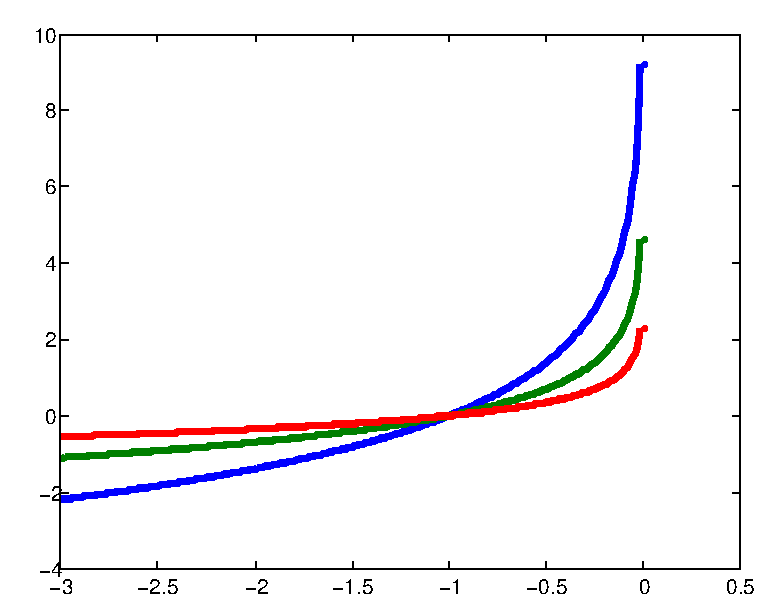
\includegraphics[width=0.8\textwidth]{images/logbarrier_cropped.pdf}
 \label{fig:1}
\end{figure}
As is easily seen, as $t$ increases the approximation becomes better.
An approximation to the nonsmooth problem is given by the following equality constrained problem,
\begin{align*}
\begin{split}
\minimize & f(\vct{x})-\sum_{i=1}^{m} \frac{1}{t}\log(f_i(\vct{x}))\\
\subjto & \mtx{A}\vct{x}=\vct{b}.
\end{split}
\end{align*}
The domain $\mathcal{D}$ of this problem is the set of points such that the inequalities $f_i(\vct{x})<0$ are strictly satisfied. One can also verify that the objective function is convex, giving rise to a convex optimization problem.
The function
\begin{equation*}
 \varphi(\vct{x}) = -\sum_{i=1}^m \log(f_i(\vct{x}))
\end{equation*}
is called the {\em logarithmic barrier function} of the system of inequalities $f_i(\vct{x})<0$: the reason is that it prevents candidates $\vct{x}$ from becoming too close to the boundary of the feasible set by becomming very large near it. With this notation, we can write the approximate problem as
\begin{align}\label{eq:logbarrier}
\begin{split}
\minimize & tf(\vct{x})+\phi(\vct{x})\\
\subjto & \mtx{A}\vct{x}=\vct{b}.
\end{split}
\end{align}
Note that here we multiplied the objective with $t$, which does not change the optimal points (but the values).
For reference, we record the gradient and Hessian of $\varphi$,
\begin{align*}
 \nabla \phi &= \sum_{i=1}^m \frac{1}{-f_i(\vct{x})}\nabla f_i(\vct{x})\\
 \nabla^2\phi &= \sum_{i=1}^m \frac{1}{f_i^2(\vct{x})}\nabla f_i(\vct{x})\nabla f_i(\vct{x})^{\trans}+\sum_{i=1}^m \frac{1}{-\nabla f_i(\vct{x})}\nabla^2 f_i(\vct{x}).
\end{align*}

 Two questions are of importance:
\begin{enumerate}
 \item How well does a solution of~\eqref{eq:logbarrier} approximate one of~\eqref{eq:constr}, and
 \item How do we solve~\eqref{eq:logbarrier}?
\end{enumerate}

\section{The central path}
The set of solutions $\vct{x}^*(t)$ of~\eqref{eq:logbarrier} for $t>0$ is called the {\em central path}. Points on the central path are strictly feasible: they satisfy $\mtx{A}\vct{x}^*(t)=\vct{b}$ and $f_i(\vct{x}^*(t))<0$. Moreover, by the Lagrange multiplier theorem, they satisfy the optimality condition
\begin{equation*}
 t\nabla f(\vct{x})+\nabla \phi(\vct{x})+\mtx{A}^{\trans}\mtx{\mu}^*=\zerovct
\end{equation*}
for some suitable Lagrange multipliers $\vct{\mu}\in \R^p$. An important property of the central path is that we can derive dual points $(\vct{\lambda}^*,\vct{\mu}^*)$, and therefore (by Lagrange duality) lower bounds on the optimal value $p^*$ of~\eqref{eq:constr}, from any point $\vct{x}^*$ on the central path. In fact, the central path can be derived from the solutions of a variant of the KKT conditions.

\begin{lemma}
 A point $\vct{x}$ is equal to a point $\vct{x}^*(t)$ on the central path if and only if there exist dual multipliers $\lambda$ and $\mu$ such that the following conditions are satisfied.
 \begin{align*}
\begin{split}
  \vct{f}(\vct{x}^*) & \leq \zerovct\\
  \mtx{A}\vct{x}^* & = \vct{b}\\
  \vct{\lambda}^*&\geq \zerovct\\
  -\lambda_i^*f_i(\vct{x}^*) & =\frac{1}{t}, \ 1\leq i\leq m\\
  \nabla_{\vct{x}} f(\vct{x}^*)+\sum_{i=1}^m \lambda_i^* \nabla_{\vct{x}}f_i(\vct{x}^*)+\mtx{A}^{\trans}\vct{\mu}^* &= \zerovct,
 \end{split}
 \end{align*}
\end{lemma}

The proof is left as an exercise. Note the analogy with the definition of the central path in the case of linear programming! Accordingly, the solution methods discussed in the context of linear programming carry over to the nonlinear case. We conclude by sketching the {\em barrier method}.

\begin{enumerate}
 \item Start with a strictly feasible $\vct{x}$ and $t:=t^{(0)}>0$, $\mu>1$ and tolerance $\e>0$;
 \item Compute $\vct{x}^*(t)$ by minimizing $tf+\phi$ subject to $\mtx{A}\vct{x}=\vct{b}$, starting with $\vct{x}$;
 \item Update $\vct{x} = \vct{x}^*(t)$;
 \item Stop if $m/t<\e$, otherwise set $t:=\mu t$ (increase $t$).
\end{enumerate}

The only unexplained part is how to solve the equality constrained minimization problem. One way is to use Newton's method on the optimality conditions of this problem.

% %-----------------------------------------------------------------------
% % End of chap1.tex
% %-----------------------------------------------------------------------


%\appendix
%\include{appendix1}

%\backmatter
%\include{biblio}
%\include{index}
\end{document}

%-----------------------------------------------------------------------
% End of chapter.tex
%-----------------------------------------------------------------------
